\documentclass[a4paper,11pt]{article}
\usepackage{color}
\usepackage{graphicx}
\usepackage{subcaption}
\usepackage{wrapfig}
\usepackage[export]{adjustbox}
\usepackage{geometry}
\usepackage{setspace}
\doublespacing
\geometry{legalpaper, portrait, margin=2cm}
\begin{document}
\title{Open Science Hardware Setup for investigating the Stability of Organic Solar Cells - Interim Report}
\author{Samuel Mendis}
\date{\today}
\maketitle
\pagebreak
\section{Introduction}
Solar cells are becoming an increasingly important factor in the fight against climate change. Silicon solar cells are the industry standard being used worldwide in a multitude of applications. Organic solar cells are showing potential to become an integral part for the  This report will outline the current development of the open hardware setup being designed to investigate the stability of organic solar cells. This project 
\section{Where the project is?}
Currently the project is at the manufacturing stage. A full design has been completed for the testing container pictured in (figure 1) which as completed using the open source software OpensCAD. As mentioned in the introduction, being an open hardware project is one of the key aspects, thereby forcing the choice of an open-source CAD software. OpensCAD was chosen as it satisfied this parameter as well the bonus of having extensive documentation allowing the designs to be completed with relative ease. Once the software was chosen, the next steps were to decide on the size and shape of the container. One of the Advanced Functional Materials Department (AFMD) researchers named () had already developed some type of testing container which is where inspiration was drawn from. 
\begin{figure}[h]

\begin{subfigure}{0.5\textwidth}
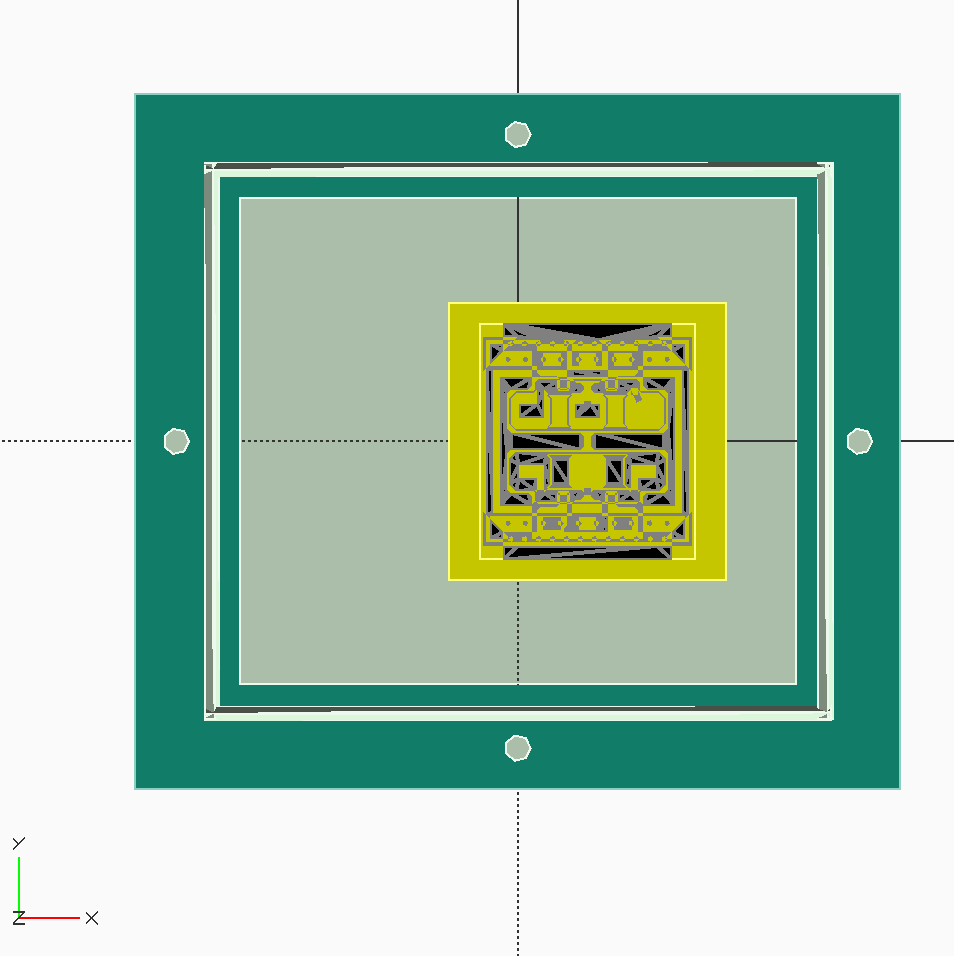
\includegraphics[width=0.9\linewidth]{fig1a}
\caption{Plan View of Model}
\label{fig:subim1}
\end{subfigure} 
\begin{subfigure}{0.5\textwidth}
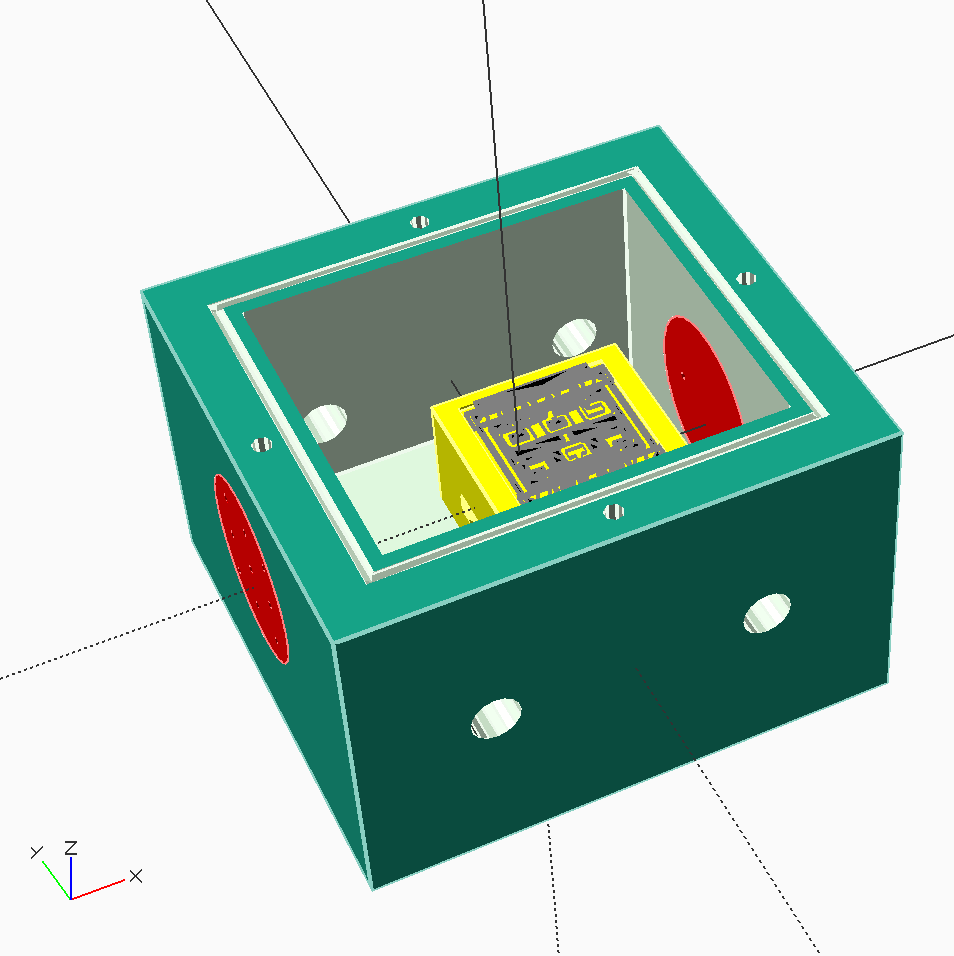
\includegraphics[width=0.9\linewidth]{fig1b}
\caption{Isometric View of Model}
\label{fig:subim2}
\end{subfigure}
\caption{Showing plan and isometric view of the full OpenSCAD model}
\label{fig:image2}
\end{figure}
\\
\\
Initially a square box was chosen with very little room inside for the implementation of devices other than the substrate. The substrate used carries 8 solar cells with dimensions of 30 mm * 30 mm and a thickness of 1 mm, this can be seen in figure (2) which is a model of the substrate used provided by Dr. Grey... To cary the substrate in the container a substrate holder was designed to fit within the outer shell of the container allowing a more modular design for the container. This modular design is desirable as it allows the ability to modify the cells which are being tested without the redesign of the entire container, just a the parts needed, thereby saving those who may need to use it in the future valuable time and money. 
\\
\\
Following the design of the model, prototypes were 3D printed in Acrylonitrile butadiene styrene (ABS) using the faculties 3D printing facilities to ensure all the parts were the correct sizes and fitted with the purchased components. The purchased components can be found in table 1 showing the part, supplier, price and function. These components were bought in, rather than manufactured, as these specific components are widely available worldwide thereby making it far more cost effective to buy from a supplier who creates the components in bulk, rather than creating bespoke parts in-house. 
\\
\\
The next important decision was what materials the container would be made from. The main objectives were to be corrosion resistant, lightweight and strong which is why Aluminium alloys were chosen as a good starting point for the outer shell. Research was undertaken to narrow the list down to four different alloys: Al-1100, Al-2011, Al-3003 and Al-5052 whose properties are listed in table 2.


As can be seen these alloys are similar in most aspects meaning the only differentiator would be cost. After contacting the University workshops, they recommended the use of x alloy for the lowest cost. Once the material for the outer shell was chosen, the next objective was to decide on which material would be used for the window. After consultation with the AFMD research group it was clear that the material used for the window had to allow UV wavelengths through narrowing the choice down to quartz. Quartz is a good transmitter of UV light allowing the solar cell to experience solar conditions which would be experienced on earth - following the AM1.5. The quartz transmission graph is shown in figure x+1 



\end{document}